% use "pdflatex -output-directory=../output Math-Notes.tex" to compile for git (assuming your in . directory)
\documentclass{report}

\input{preamble}
\input{macros}
\input{letterfonts}

\title{\Huge{Math}\\Notes}
\author{\huge{By me (Thanks to for the template \href{https://github.com/SirCharlieMars/dotfiles/tree/master/latex_template}{SirCharlieMars})}}
\date{}

\begin{document}

\maketitle
\newpage% or \cleardoublepage
% \pdfbookmark[<level>]{<title>}{<dest>}
\pdfbookmark[section]{\contentsname}{toc}
\tableofcontents


\pagebreak % 1.1


\chapter{Algebra}
\section{Indices}

\dfn{Index Laws}{
    \begin{enumerate}
        \item $a^m \times a^n = a^{n + m}$
        \item $a^m \div a^n = a^{n - m}$
        \item $(a^m)^n = a^{m \times n}$
        \item $a^{-m} = \frac{1}{a^m}$
        \item $a^0 = 1$
        \item $a^{\frac{m}{n}} = \sqrt[n]{a^m}$
    \end{enumerate}
}

\ex{Laws In Action}{
    \begin{enumerate}
        \item $2^3 \times 2^7 = 2^{10}$
        \item $\frac{3^6}{3^2} = 3^4$
        \item $(5^2)^5 = 5^{10}$
        \item $7 \times 2^{-2} = \frac{7}{2^2}$
        \item $45^0 = 1$
        \item $5^{\frac{-3}{7}} = \frac{1}{\root 7 \of {5^3}}$
    \end{enumerate}
}
\nt{Indices are used extremely frequently and there are often multiple laws hidden in each question}


\pagebreak % 1.2


\section{Logarithms (Logs)}

\dfn{Principle}{The general equation is: \[log_{(a)}(y) = x \leftrightarrow a^x = y\]\\For example:\[log_{10}1 = 0 \leftrightarrow 10^0 = 1\]\\To calculate logarithm: \[\frac{log_{(10)}(y)}{log_{(10)}(a)}\]}
\dfn{Laws}{
    \begin{enumerate}
    %% contains in and out of brackets
        \item $\log_{(a)}(x) + \log_{(a)}(y) = \log_{(a)}(xy)$
        % \item $\log_{a}x + \log_{a}y = \log_{a}xy$
        \item $\log_{(a)}(x) - \log_{a}(y) = \log_{(a)}(\frac{x}{y})$
        % \item $\log_{a}x - \log_{a}y = \log_{a}\frac({x}{y})$
        \item $\log_{(a)}(x^n) = n\log_{(a)}(x)$
        % \item $\log_{a}x^n = n\log_{a}x$
        \item $\log_{(a)}(a) = 1$
        % \item $\log_{a}a = 1$
        \item $\log_{(a)}(1) = 0$
        % \item $\log_{a}1 = 0$
    \end{enumerate}
    To use these laws, the bases must be the same $a$
}

\ex{Laws In Action}{Round to two decimal place
    \begin{enumerate}
        \item $\log_{2}2 + \log_{2}5 = \log_{2}10 = 3.32$
        \item $\log_{5}12 - \log_{5}2 = \log_{5}6 = 1.11$
        \item $\log_{7}{2^2} = 2 \times \log_{7}2 = 0.71$
        \item $\log_{84}84 = 1$
        \item $\log_{153}1 = 0$
    \end{enumerate}
}

\nt{some calculators have a default log base of 10, this means $\log_{10}(x) = \log_{}(x)$}


\pagebreak


\section{Quadratic Equations}

\dfn{Formulae}{A quadratic equation is an equation where the highest power is two.\\The standard form quadratic equation: \[ax^2 + bx + c = 0\] where $a,b,c$ are known.\\The quadtratic formula (can only be used by standard form equations):\[x = \frac{-b \pm \sqrt{b^2-4ac}}{2a}\]\\Completing the square \[ax^2 + bx + c = 0\rightarrow \]\\The porabola:\[y = ax^2 + bx + c\]}


\chapter{Trigonometry}
\section{Right-Angled}
\dfn{Identification}{A triangle is right-angled if it contains a right angle ($90^\circ$): $$
\begin{tikzpicture}
    \draw  (0, 0) coordinate (A)
    -- node[left] {} (0,2) coordinate (C)
    -- node[above right] {} (3,0) coordinate (B)
    -- node[below] {}  (0, 0);
    \draw (0,10pt) -- ++(10pt,0) -- ++(0,-10pt);
    \node at (A)[anchor=north] {};
    \node at (B)[anchor=north] {};
    \node at (C)[anchor=south] {};
\end{tikzpicture}$$
}
\dfn{Formulae}{Pythagorean theorem $c^2 = a^2 + b^2$ can find the exact length of the an unknown side given two other known sides.\\\\Trigonometric Ratios are:\\\\Sine:$$\sin\theta = \frac{o}{h}$$\\Cosine:$$\cos\theta = \frac{a}{h}$$\\Tangent:$$\tan\theta = \frac{o}{a}$$\\Where $o$ is the opposite leg $a$ is the adjacent leg, $h$ is the hypotenuse, $\theta$ is the angle.$$
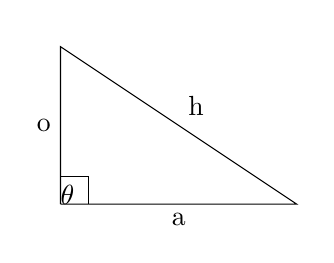
\begin{tikzpicture}
    \draw  (0, 0) coordinate (A)
    -- node[left] {o} (0,2) coordinate (c)
    -- node[above right] {h} (3,0) coordinate (b)
    -- node[below] {a}  (0, 0) coordinate (a);
    \draw (0,10pt) -- ++(10pt,0) -- ++(0,-10pt);
    \node at (a)[anchor=north] {};
    \node at (b)[anchor=north] {};
    \node at (c)[anchor=south] {};
    {angle = b--a--c};
    pic["$\theta$"]
\end{tikzpicture}$$ % fix broken theta
}
\nt{To remember the Trigonometric ratios, we can use $SOHCAHTOA$.} % SOHCAHTOA explanation later

\pagebreak

\section{Non-Right-Angled}

% TODO: surds
% TODO: exact triangles



\end{document}
